\cleardoublepage
\newrefsection
\chapter{文献综述}

\section{背景介绍}

RISC-V 处理器凭借其低成本与生态优势，在物联网、嵌入式以及高性能计算领域获得了广泛的应用。
但是随着应用范围的扩展，RISC-V 处理器也面临着严重的安全威胁。
其中，侧信道攻击是一种利用处理器微架构状态来窃取计算机系统中机密信息的攻击方式，造成极大安全隐患。
形式化验证可以在处理器设计阶段发现侧信道漏洞。
这一章我们将对RISC-V处理器、侧信道漏洞与形式化验证进行简单介绍。


\subsection{RISC-V 处理器}

RISC-V 是一种开源的精简指令集架构（ISA），在学术界和工业界得到了广泛的应用。
该 ISA 由一个基本的整数指令集与若干拓展指令集如乘除法扩展、原子扩展、浮点扩展等构成。
RISC-V 处理器是可以执行全部或者部分 RISC-V 指令集的硬件实现。

RISC-V 处理器的开发者根据性能，安全等需求，设计不同的硬件实现，即微架构。
常见的 RISC-V 微架构可以分为轻量级，应用级和高性能三种类型。
轻量级通常采用简单的单发射、顺序执行以及极短的流水线设计，开源代表为 Ibex 处理器；
应用级微架构通常采用多流水线、乱序发射技术，开源代表为 CVA6\cite{zaruba2019cost} 处理器；
高性能微架构采用复杂的超标量、乱序执行、深度流水线及多级分支预测技术，开源代表为 BOOM\cite{zhaosonicboom} 处理器。

\begin{figure}
    \centering
    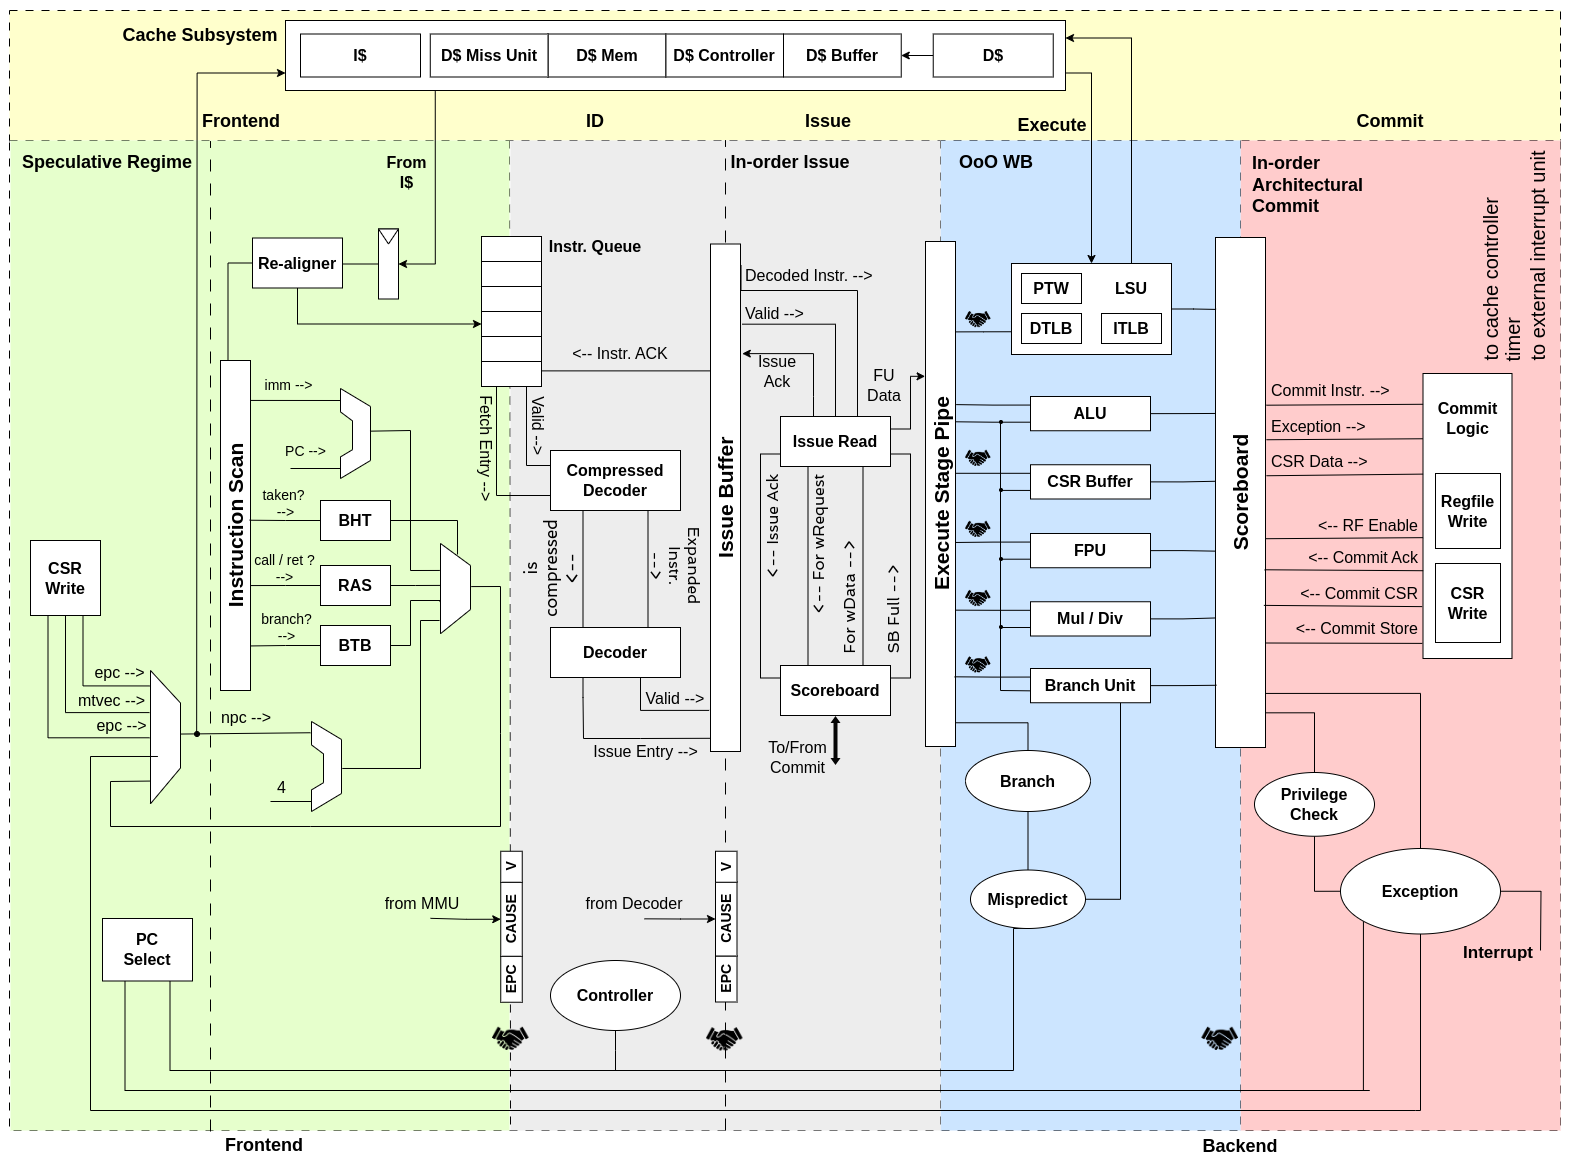
\includegraphics[width=0.85\textwidth]{figure/review/cva6.png}
    \caption{CVA6 处理器微架构图}
    \label{fig:cva6}
\end{figure}

为了提升处理器性能，RISC-V 处理器引入了若干微架构设计。
图\ref{fig:cva6} 是 CVA6 处理器的微架构图。
以 CVA6 为例：分支历史表（BHT）根据历史分支指令的跳转结果做出分支预测，减少分支预测错误的惩罚；
返回地址栈（RAS）记录函数调用链的返回地址，加速函数调用的返回过程；
缓存（Cache）保存频繁读取的内存数据，减少内存访问次数；
计分板（Scoreboard）进行指令的乱序发射，并将前序指令的计算结果进行前递，降低了指令之间的数据冲突。


\subsection{侧信道攻击}

侧信道攻击指利用处理器在运行过程中的物理泄露或微架构状态来窃取计算机系统中的机密信息。
本文主要关注利用处理器微架构的侧信道攻击。
现代处理器微架构为了追求高性能，广泛使用 Cache，BTB 等微架构部件来提高指令执行效率。
例如，缓存命中（Cache Hit）可以节约几十个时钟周期的访存时间开销。
所以即使执行同一条指令，也有可能因为微架构状态的不同，从而使得指令执行的时间出现差异。
程序中不同机密数据的值参与计算会在微架构上留下不同的状态。
所以攻击者可以根据指令执行行为的差异，推测出微架构的状态，从而推测出机密数据的值。

侧信道攻击可以分为微架构状态编码和微架构状态解码两个阶段。
在微结构编码阶段，受害者会读取机密数据进行某些运算，这些运算会对微架构状态产生改变；
或者是攻击者通过架构不可见的方式读取机密数据，并将机密数据固定在微架构状态中。
在微架构解码阶段，攻击者通过某些原语\cite{184415}，将微架构状态恢复为架构可见的值。

侧信道攻击可以分为三种类型：瞬态执行攻击、指令恒定时间执行攻击和计时器无关攻击。

1. 瞬态执行攻击利用现代处理器的推测执行或异常延迟处理，投机执行某些本不会被执行的代码。
攻击者通过训练分支预测器\cite{8835233}、毒害返回地址栈\cite{10.1145/3243734.3243761}、人为触发异常\cite{10.1145/3357033}、
制造端口争用\cite{10.1145/3319535.3363194}或微架构采样\cite{10.5555/3277203.3277277}来打开瞬态执行窗口。
在这个瞬态执行窗口中，处理器会根据攻击者的意图执行某些代码片段。
这些代码的执行结果虽然会被撤销，但是却将某些机密信息编码到了微架构中，例如 Cache。
这些编码了机密信息的微架构就可以作为侧信道，解码机密信息。

2. 指令恒定时间执行攻击是一种利用指令执行时序差异来窃取机密信息的侧信道攻击。
现代处理器为了效率最大化，会在硬件电路上对整数除法、浮点运算等运算单元进行时序优化\cite{10.5555/3698900.3699201}\cite{10.5555/3620237.3620638}。
导致这些指令执行所需的时钟周期（Clock Cycles）严格依赖于输入操作数的具体数值。
如果在处理机密信息时使用了非恒定时间执行的指令，攻击者便可以通过测量指令执行时间，并将其映射为机密数据的值，
从而实现信息窃取。

3. 计时器无关攻击\cite{10.1145/3719027.3744833}不依赖计时器来解码微架构中的状态信息。
在传统的侧信道攻击中，通常需要使用高精度的计时器来测量微架构状态的差异。
现代的处理器为了防御侧信道攻击，很多不再提供高精度的计时器。
而计时器无关的侧信道攻击在微架构解码阶段无需使用计时器，而是利用一种原子指令原语。
这种原语可以将缓存状态反映到架构寄存器上，提供了一种新的微架构状态解码方式。


\subsection{形式化验证}
形式化验证是一种基于严格数学基础的系统正确性分析与验证技术。
其通过静态的符号化或穷举的方式遍历待验证对象的全局状态空间，能够以数学上的完备性覆盖所有可能的执行路径与输入组合。
形式化验证被应用到处理器设计上，用于验证处理器是否存在侧信道漏洞\cite{10.1145/3658644.3690344}\cite{10.1145/3613424.3614254}。
一般来说，针对处理器的形式化验证分为以下四步进行：

1. 确定验证对象。处理器设计形式化验证需要指定顶层模块，一般选用处理器核心作为顶层模块。
顶层模块的输入会被形式化验证引擎抽象为符号值，代表其为任意输入。

2. 编写安全属性。形式化验证的核心是验证一个系统是否满足某些属性。
验证者需要提取系统的的安全规范，将其形式化为一组精确的安全属性。
具体来说，安全属性是待验证系统中的某几个变量的值在时序或者逻辑上应该满足的某些恒等关系。
一般使用 SystemVerilog Assertions\cite{10.5555/2677118} 进行编写。
语法体系自底向上划分为布尔表达式、序列与属性三个抽象层次。
% 针对侧信道攻击来说，安全属性一般定义为：两条相同的指令提交时间必须一致，并且内存总线上不应该出现机密信息的地址\cite{10.1145/3669940.3707243}。

3. 选择验证引擎。形式化验证引擎是实现严格数学证明的核心算法。
在底层架构上，现代验证引擎通常使用布尔可满足性（SAT）求解器或可满足性模理论（SMT）求解器。
在验证执行过程中，引擎将处理器RTL代码精确抽象为数学状态转换系统，同时将安全属性转化为时序逻辑命题。
引擎随后在全局状态空间内穷举所有可能的输入序列。
根据求解目标是证明或者证伪，有界或者无界来选择基于不同数学算法的求解引擎。

4. 分析验证结果。形式化验证具有完备性。
如果某个安全属性被证明了，则说明不存在一种输入违反该安全属性。
反之，如果某个安全属性被证伪，形式化验证引擎会给出一个反例。该反例可以触发安全属性违例。
但是形式化验证也有可能出现超时的结果，即在给定的时间内无法证明或证伪。


\section{国内外研究现状}

处理器侧信道漏洞的形式化检测作为处理器的形式化验证的一种应用场景，流程与传统处理器的形式化验证相似。
本章从验证对象的边界，待验证的安全属性与同步状态的定义三方面介绍针对处理器侧信道漏洞的形式化验证。

\subsection{研究方向及进展}

\subsubsection{验证对象的边界}
在形式化检测中，验证对象的边界直接决定了漏洞挖掘的精确度以及遭遇状态空间爆炸的几率。
InSpectre\cite{10.1145/3372297.3417246}，Hardware-Software Contracts\cite{9519500} 和 CheckMate\cite{8574598} 为了规避底层硬件巨大的状态空间，
选择不以任何RTL代码作为求解顶层，而是构建一个包含乱序或推测执行特征的数学状态机模型。
这种抽象能够从更高维度快速证明或证伪特定的预测执行机制

这类抽象模型由于脱离了具体的RTL连线与逻辑门，无法发现因特定总线竞争、有限状态机错误等底层实现缺陷导致的侧信道漏洞。
AutoCC\cite{10.1145/3613424.3614254} 将验证对象转移到真实的RTL代码上。
该框架的顶层边界可以是单独的如 AES 加速器的硬件加速器，或者是经过黑盒化处理的简单处理器核心。
当以处理器核心为顶层时，为了让求解器能在合理时间内跑出结果，AutoCC 建议将内部状态过于复杂的子模块作为黑盒移出验证边界。

$\mu$CFI\cite{10.1145/3658644.3690344} 将其验证顶层设定为顺序执行的处理器核心，如 Ibex，PicoRV32 等。
整个CPU的所有流水线阶段均在求解边界之内，成功发现了 Ibex 处理器内部乘法器与异常处理模块之间的侧信道。
Contract Shadow Logic\cite{10.1145/3669940.3707243} 将边界进一步拓展到了复杂的乱序执行处理器核心。
该工作的验证顶层包含了两份完整的乱序核心RTL代码以及辅助验证的影子逻辑。
但是现代形式化求解引擎难以对复杂乱序处理器进行求解，通常需要进行一定的状态空间裁剪。
Contract Shadow Logic 使用影子逻辑过滤了部分求解需求。


\subsubsection{待验证的安全属性}
针对微架构侧信道，研究者们将安全属性进行定制与拓展。
在 InSpectre\cite{10.1145/3372297.3417246} 中，作者提出了条件非干扰性。
即证明处理器在引入乱序和预测执行等优化后，不会比纯顺序执行的参考模型泄露更多的信息。
类似地，Hardware-Software Contracts\cite{9519500} 中定义了推测非干扰性。
要求程序在顺序执行时不可区分的状态，在投机执行下也必须对攻击者不可区分。可以形式化地表示为：
$$\forall P,\ M_{pub},\ M_{sec},\ M'_{sec}$$
$$\mathbf{if}\ O_{ISA}(P,\ M_{pub},\ M_{sec})\ =\ O_{ISA}(P,\ M_{pub},\ M'_{sec})$$
$$\mathbf{then}\ O_{\mu Arch}(P,\ M_{pub},\ M_{sec})\ =\ O_{\mu Arch}(P,\ M_{pub}, M'_{sec})$$


Hardware-Software Contracts\cite{9519500} 的该安全属性从软硬件层面解释为：
如果两条同样的指令对架构上的影响相同，那么这两条指令对微架构的影响也应该相同。
即，如果软件满足特定的沙盒约束或恒定时间编程约束，则硬件承诺在此契约下不发生泄露。
Contract Shadow Logic\cite{10.1145/3669940.3707243} 直接将该安全属性转化为 RTL 级别的断言进行求解。
AutoCC\cite{10.1145/3613424.3614254} 使用了该安全属性的变体，观察微架构的差异能否引起架构的差异。


$\mu$CFI\cite{10.1145/3658644.3690344} 不再局限于传统的计时侧信道，而是定义一种信息流安全属性：
处理器在时钟周期级别的程序计数器（PC）轨迹，只能被 ISA 明确允许的指令操作数影响。
该属性统一了微架构侧的恒定时间执行与控制流劫持漏洞检测，将时序侧信道问题转化为了针对 PC 的污点追踪安全性断言。

\subsubsection{同步状态的定义}

在抽象模型层面，Hardware-Software Contracts\cite{9519500} 和 InSpectre\cite{10.1145/3372297.3417246} 通过数学关系，如不可区分性关系，来定义同步。
它们在每个求值步骤中，要求两个实例在相同的检查点达成一致。

在 AutoCC\cite{10.1145/3613424.3614254} 中，同步状态被明确定义为硬件冲刷（Flush）。
工具强制两个实例在受害者进程结束、刷新机制执行完毕后达成状态同步，即拥有相同的架构状态。
随后，在给定的稳定周期后启动间谍进程，比较两者的微架构状态输出是否分化。

在乱序处理器中，缓存命中与缺失会导致两个实例失去同步。
Contract Shadow Logic\cite{10.1145/3669940.3707243} 通过引入两阶段影子逻辑解决这一问题。
当两个实例的微架构轨迹发生分化时，系统进入第二阶段，此时影子逻辑通过暂停较快实例的时钟，强制两个实例在指令提交当拍阶段实现周期对齐。
这种物理级别的同步状态定义，解决了乱序处理器中异步提交导致的假阳性问题。

$\mu$CFI\cite{10.1145/3658644.3690344} 基于单实例的门级信息流追踪，绕过了双实例的同步过程。

\subsection{存在问题}



\section{研究展望}

\newpage
\begingroup
    \linespreadsingle{}
    \printbibliography[title={参考文献}]
\endgroup
